\newpage
\newpage
[.]
\pagebreak

\section{Extreme value theory}
\label{sec:evt}
\subsection{Background}
The mean SSH will
not be able to damage the coast; life and property will only be put
at risk by the most extreme events above that~\cite{taleb2019statistical, Taleb2012AntifragileH}.
Extreme value theory (EVT) is the provides the necessary tools
to look at the return period of extreme events of a certain value.
The two primary EVT methods are Peak over Threshold
(POT)\footnote{Y20~\cite{ZannaPreprint} used POT methods. } and Block Maxima (BM).
Both of these strategies require
large amounts of data to converge~\cite{taleb2019much} (e.g.~\texttt{c50}).
BM leads to Generalised Extreme Value (GEV) distribution:


    \(
    \operatorname{GEV}(\mu, \sigma, \xi):
    \)

    \(
    \text{ location, position of the GEV mean } \mu \in \mathbb{R};
    \)

    \(
    \text{scale, } \sigma>0;
    \)

    \(
    \text{shape, } \xi \in \mathbb{R}.
    \)

    \iffalse
    \begin{align}
        \chi(x)=&\{
               \begin{array}{ll}
                    \left(1- \xi\left(\frac{x-
                    \mu}{\sigma} \right)\right)^{\frac{1}{\xi}} &
                     \text { if } \xi \neq 0 \\
                    e^{-\frac{x-\mu}{\sigma}} &
                    \text { if } \xi=0 \\

              \end{array}.
    \tag{GEV-2} \label{eq:GEV-2}

    \end{align}
    \fi

\begin{align}
    \operatorname{GEV}(x; \mu, \sigma, \xi)=&
    \frac{1}{\sigma} \chi(x)^{1-\xi} e^{-\chi(x)}; \tag{GEV-1}
    \label{eq:GEV-1}\\
    \chi(x)=&\left\{\begin{array}{ll}
    \left(1-\xi\left(\frac{x-\mu}{\sigma}\right)\right)^{1 / \xi} & \text { if } \xi \neq 0 \\
    e^{-(x-\mu) / \sigma} & \text { if } \xi=0 \tag{GEV-2}
    \end{array}\right.
   \label{eq:GEV-2}
\end{align}


    A GEV with $\xi>0$, $\xi=0$, $\xi<0$ are
    respectively called the Weibull, Gumbel, and Fr\'echet
    distributions.\footnote{Here I have used the opposite sign convention for
    the shape, $\xi$, than is more commonly used. Please check against the
    forms of \ref{eq:GEV-1}~\&~\ref{eq:GEV-2} before interpreting results. }

\subsection{Block maxima GEV}
The highest SSH value in a given year at a given point
is extracted from \texttt{control-1950}, yielding 101 values per point.
It was decided not to subtract the seasonal SSH cycle from these
values, as it is the absolute height of the sea surface which
creates the hazard rather than the relative height.

\begin{figure*}[htb!]
    \centering
    \includegraphics[width=0.8\linewidth]{../surge/plots/GEV_modelNO.pdf}
    %\vspace{-25pt}
   \caption{New Orleans GEV plot for \texttt{control-1950} Interesting transition
            - does this represent hurricanes?}
    \label{fig:gev-no}
    \includegraphics[width=0.8\linewidth]{../surge/plots/skextreme_second_tactic.pdf}
    \vspace{-15pt}
   \caption{Confidence intervals not defined near Miami and Eastport. }
    \label{fig:gev_all_points}
\end{figure*}


\begin{figure*}[htb!]

\begin{minipage}{0.45\textwidth}

\includegraphics[width=1\linewidth]{../surge/plots/GEV_pi_plateau_NO.pdf}
\caption{First attempt at enforcing a GP asymptote of 2m for New Orleans,
with an \texttt{RBF} kernel.
The data is the same as in Figure~\ref{fig:gev-no}. The
kink is caused by using a non-differentiable mapping to
enforce the far-field conditions. 1$\sigma$ and 2$\sigma$ envelopes shown.}
\end{minipage}
\begin{minipage}{0.45\textwidth}

    \centering
    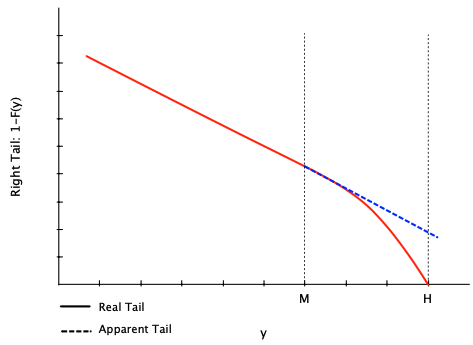
\includegraphics[width=1\linewidth]{images/taleb-limit-slimmed.png}\\
    \textit{Figure 15.1 from T19~\cite{taleb2019statistical} p.~279}
   \caption{As shown if you only
   observe a distribution up to some value M,
    you may be tempted to fit a line through the
   data (dotted blue line).
   But if there were in fact a limit to the distribution at H,
   you would be overestimating
   the true number of very extreme events (red curve),
   predicting events that were larger than were possible.}
   \label{fig:up-bound-taleb}
   \end{minipage}

   \begin{minipage}{0.45\textwidth}
   \centering
   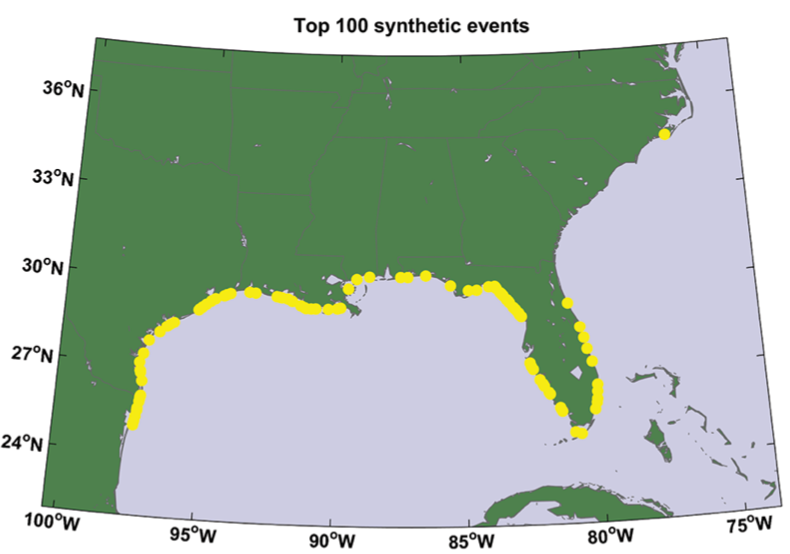
\includegraphics[width=1\linewidth]{images/top-100-landfalls.png}\\
   \textit{Figure 3b from \cite{emanuel2017will}}
   \caption{The top 100 most rapidly intensifying events in the model,
   showing that models capture far more of these TCs in the Gulf of Mexico
   and Florida than further north.
     }
   \label{fig:top-100}
   \end{minipage}
   \begin{minipage}{0.45\textwidth}
   \centering
   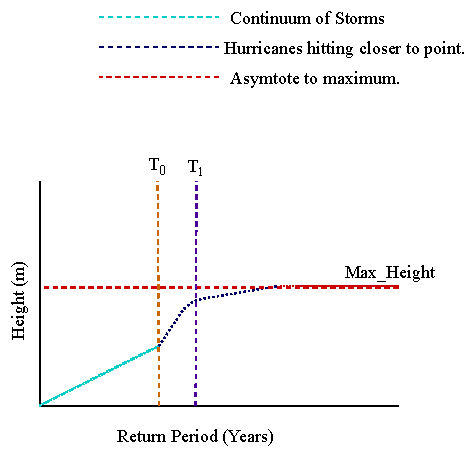
\includegraphics[width=1\linewidth]{images/Return_Hypothesis.pdf}
   \vspace{-15pt}
  \caption{The maximum height is a function of the potential intensity
  allowed by the climate, and the responsiveness of that point on the coastline to a
  wind stress of that size. If T$_0$, or T$_1$, is a similar or greater than the time period of
  measurement, then it is respectively possible that no hurricanes exist in the data sample,
  or that no hurricanes make direct landfall at that location.}
    \label{fig:return_hyp_new}
    \end{minipage}





\end{figure*}



Using my adaptation of \texttt{skextremes}~\cite{skextremes} I fit the
GEV using maximum likelihood estimation.\footnote{with an initial guess from \texttt{lmoments}, optimised using
\texttt{scipy.stats.genextreme} with \texttt{scipy.optimize.fmin\_bfgs}~\cite{2020SciPy-NMeth}.}
For some confidence interval, $\alpha$, the Gaussian confidence interval of the parameters is
estimated by the Delta method~\cite{coles2001introduction},

\begin{equation}
[\Delta \sigma , \Delta \mu, \Delta \xi] =
\mathcal{N}^{-1}(1-\frac{\alpha}{2}; 0, [\sigma_e (\sigma), \sigma_e (\mu), \sigma_e (\xi)])
\end{equation}

where,

\begin{equation}
[\sigma_e (\sigma), \sigma_e (\mu), \sigma_e (\xi)] =
\mathrm{sqrt}\left(\mathrm{diag}\left(\left( \mathrm{Hess}([\sigma, \mu, -\xi]) \right)^{-1} \right)\right).
\end{equation}

and $\mathcal{N}^{-1}(x; \mu_n, \sigma_n^2)$ is the inverse normal distribution
with input $x$, and parameters $\mu_n$,\& $\sigma_n^2$.

For a period of time $T$, we can define a value $\phi$:

\begin{equation}
\phi \equiv - \log(1 - T_{r}/T)
\end{equation}

where $T_r$ is the sampling time of BM (1 year).

$E$, the size of the largest value expected at that time $T$:

\begin{equation}
\mathbb{P}(X>E) \equiv \frac{T_r}{T}
\end{equation}

where $\mathbb{P}$ is the probability which we have assumed is
distributed as a GEV.

We then then work out the uncertainty in each point in the
return plot fits (Figure~\ref{fig:gev-no}C), which is asymptotically
Gaussian~\cite{doob1935limiting}.

\begin{align}
\delta \mathbf{Z} = & \left[ \begin{array}{l}(\sigma\cdot\xi^{-2} \cdot (1-(\phi^{\xi})
            \\ \sigma \cdot (\xi^{-1})\cdot (\phi^{\xi}) \cdot \log(\phi)),\\
            1,\\
            (1- \frac{\phi^{\xi}}{\xi})
            \end{array} \right]
\end{align}

\begin{equation}
\sigma_e(E) = \mathrm{sqrt}\left(\left(\delta \mathbf{Z} \cdot \left( \mathrm{Hess}\left([\sigma, \mu, -\xi]\right)
\right)^{-1} \right) \cdot  \delta \mathbf{Z}^{\mathrm{T}}\right)
\end{equation}

\begin{equation}
\Delta_e (E) = \mathcal{N}^{-1}(1-\frac{\alpha}{2}; 0, \sigma_e(E))
\end{equation}

The measured points on the return plot (e.g.~\ref{fig:gev-no}C) are $EV_i$ against $T_i$:

\begin{equation}
T_i = \frac{Ttotal}{i} ,
\end{equation}

and,

\begin{equation}
EV_i = \mathrm{sorted(Block\; Maxima\; Values)}_i.
\end{equation}

where they have been sorted from smallest to largest, where $Ttotal$ in this
case is 101 years.


Figure~\ref{fig:gev-no} fits the GEV fitted
on the yearly BM for the nearest coastal point to NO,
and Figure~\ref{fig:gev_all_points} shows the fit along all points in \texttt{eUS}
for \texttt{c50}. As can be seen, points in the Gulf of Mexico generally have  $\xi<0$ (Fr\'echet, finite lower bound),
whereas northwards it becomes more likely that $\xi>0$ (Weibull, finite upper bound).
As in Figure~\ref{fig:top-100} this could be explained by the greater incidence of
TCs, a finite amplitude instability, which would pull the MLE fit to curve up, decreasing $\xi$.


\subsection{Enforcing an asymptote using potential intensity theory }
\label{sec:evt-limit}

As noted in~§~\ref{sec:hurr-theory} there is a PI
that a TC would be able to reach given the climate.
As shown in Figure~\ref{fig:up-bound-taleb} naively fitting
the GEV would be an over-extrapolation, if we have a good physical reason for
thinking that there is a maximum
(i.e.~the PI §~\ref{sec:hurr-theory}).

Figure~~\ref{fig:return_hyp_new} suggests a hypothesis to explain the observed pattern of return periods is explained in
Figure~\ref{fig:return_hyp_new}, where the PI of TCs flattens the extreme
value against return period (see Figure~\ref{fig:eman-pi}).
If there were no TCs in the sample, this would appear as the blue curve in Figure~~\ref{fig:return_hyp_new} continued without reaching the true plateau.
The period of time between T$_0$ (the expected period a TC) and T$_1$ (the expected period a TC direct hit)
would depend on the average size of the tropical cyclone storms (c.~1000km),
and the percentage of them which rise to their PI.

Given that
the error is asymptotically Gaussian
a Gaussian process (GP)~\cite{williams2006gaussian, duvenaud2014automatic} (see §~\ref{sec:gp-theory})
could be used to fit the function (see Figure~\ref{fig:gp-plateau}), fixed so that
the asymptotic mean $\to0$ as $T\to0$, and to plateau value given the
responsiveness \& PI of the point as $T\to\infty$.

A way to falsify this hypothesis would be to use longer runs than \texttt{c50},
to prove that the deviation is caused by the length of time that BM takes to
converge to GEV, but this seems unlikely given that the Figure~\ref{fig:gev-no}C
is replicated in other locations (e.g.~Pensecola, Galverston).

\begin{table}[h!]
    \centering
    \begin{tabular}{ll}
    \hline \hline
    \textbf{Sym} & \textbf{Description} \\
    \hline
        $\sigma$ & Scale. \\
        $\xi$ & Shape. \\
        $\mu$ & Location. \\
        $\sigma_e(.)$ & The standard devation of a parameter (.)\\
        Hess & The Hessian.\\
        diag & The diagonalization of the matrix. \\
        sqrt & Element wise square root.\\
        \alpha & The significance level (at 0.05 in Figure~\ref{fig:gev-no}.)\\
        $\delta \mathbf{Z}$&  \\
        sT & \\
        sT2 & \\
    \hline \hline
    \end{tabular}
    \caption{Symbols (Sym) for extreme value theory.}
    \label{tab:fluid_variables}
\end{table}


\begin{figure}[htb!]
    \centering
    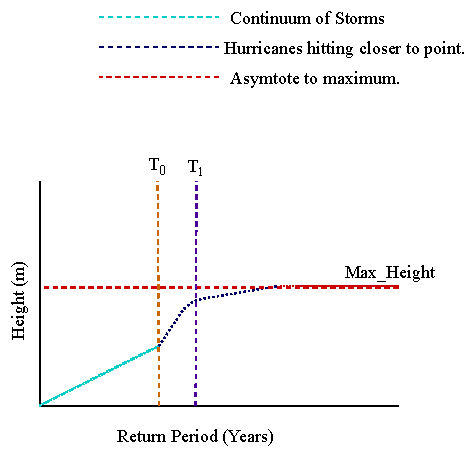
\includegraphics[width=1\linewidth]{images/Return_Hypothesis.pdf}
    \vspace{-15pt}
   \caption{The maximum height is a function of the potential intensity
   allowed by the climate, and the responsiveness of that point on the coastline to a
   wind stress of that size. If T$_0$, or T$_1$, is a similar or greater than the time period of
   measurement, then it is respectively possible that no hurricanes exist in the data sample,
   or that no hurricanes make direct landfall at that location.}
     \label{fig:return_hyp_new}

\end{figure}



\FloatBarrier
